Many of the methods proposed in this thesis proposal are inspired by the success of many computer vision techniques. For example, in Chapter-3, we use bag-of-strokes, inspired by bag-of-words method, to represent the scene text as strokes. In Chapter-4 we take the motivations from deep learning and specifically recurrent neural networks to solve the script and language identification problem in document images at word and line level. In this chapter, Section~\ref{sec:tools} details about the Bag-of-Words (\textsc{BoW}) methods and support vector machines (\textsc{SVM}) used for script identification in the wild, Section~\ref{sec:deep} details about the deep learning and recurrent neural networks used for script and language identification in document images at word and line level.

\section{Bag-of-Words(~\textsc{BoW} and \textsc{SVM})}
\label{sec:tools}

\subsection{Image Descriptors}
In computer vision, image descriptors or visual descriptors are descriptions of the visual features of the contents in images, videos, or algorithms or applications that produce such descriptions. They describe elementary characteristics such as the shape, the color, the texture or the motion, among others. Visual descriptors are divided in two main groups:
\begin{itemize}
\item Global descriptors which are computed on whole images.
\item Local descriptors which are computed locally on a small regions or point of interests on image.
\end{itemize}

In this subsection, we will describe about common image descriptors like Local Binary Pattern (\textsc{LBP}), Scale Invariant Feature Transform (\textsc{SIFT}).

\subsubsection{Local Binary Patterns ~\textsc{LBP}}
A Local Binary Pattern (~\textsc{LBP}) ~\cite{LBPOjala2002} is a local descriptor that captures the appearance of an image in a small neighborhood around a pixel. An LBP is a string of bits, with one bit for each of the pixels in the neighborhood. Each bit is turned on or off depending on whether the intensity of the corresponding pixel is greater than the intensity of the central pixel. Figure~\ref{fig:lbpPic} depicts the basic \textsc{lbp} operator.

\begin{figure}
\centering
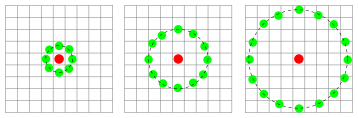
\includegraphics[scale=1]{figures/Lbp_neighbors.png}
\caption{The basic ~\textsc{lbp} operator. The figures shows the circular $(8, 1)$, $(16,2)$ and $(8,2)$ neighborhoods. The pixels are bilinearly interpolated whenever the sampling point is not at the center of a pixel. Figure source~\cite{LBPOjala2002}.}
\label{fig:lbpPic}
\end{figure}

\subsubsection{\textsc{SIFT}}
Scale-Invariant Feature Transform (\textsc{SIFT}) proposed by Lowe ~\cite{Lowe04} is one of the popular local feature detector and descriptor. SIFT descriptor is invariant to Affine transformation, Lighting changes, Noise. The original SIFT implementation includes both an interest point detector and feature descriptors at
the interest points. The descriptor associates to the regions a signature which identifies their appearance compactly and robustly. Figure 2.3 shows an example of SIFT descriptor computation at some
keypoints, and how they can be used to match points in different images. 

Computing \textsc{SIFT} descriptor at a point starts with sampling the image gradient magnitudes and orien-
tations in a region around the point. The samples are then accumulated into orientation histograms (bin
size = 8), summarizing the contents over $4 \times 4$ subregions. These orientation histograms capture the
local shape. The final descriptor is formed from a vector containing the values of $4 \times 4$ array of orientation histogram around the point. This leads to a \textsc{SIFT} feature vector with $4 \times 4 \times 8 = 128$ elements. To obtain illumination invariance, the feature vector is normalized by the square root of the sum of squared components.

\subsubsection{Gradient Based Features~\cite{Vibhor13}}
Inspired by the success of Histogram of Oriented Gradient (HOG) features~\cite{Dalal05} in many vision tasks, we adapted them to the word recognition problem. To compute the adapted HOG features, we begin by applying the Canny edge operator on the image. Note that we do not expect a clean edge map from this result. We then compute the orientation of gradient at each edge pixel. The gradient orientations are accumulated into histograms over vertical (overlapping) strips extracted from the image. The histograms are weighted by the magnitude of the gradient. An illustration of the feature computation process in shown in Fig.~\ref{fig:hogPic}. At the end of this step, we have a representation of the image in terms of a set of histograms.

\begin{figure}
\centering
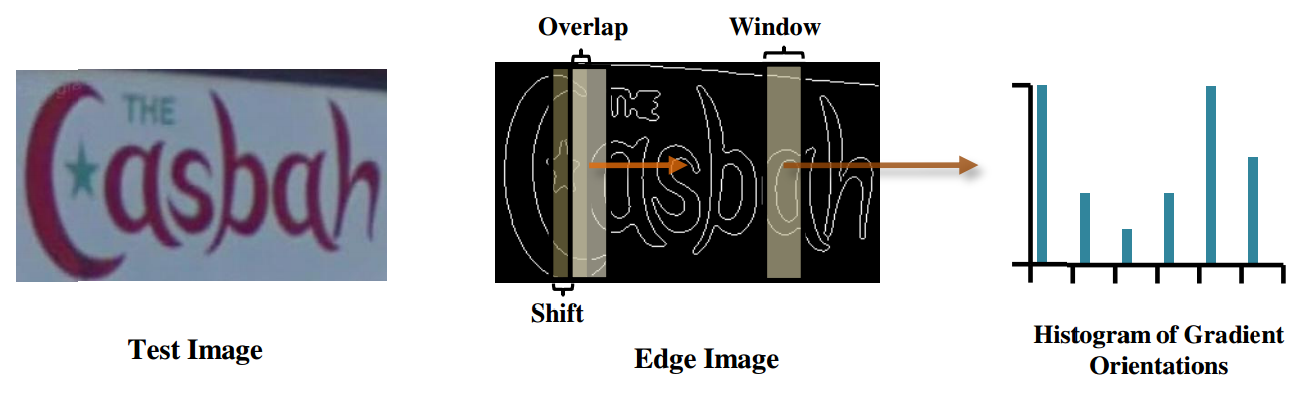
\includegraphics[scale=0.4]{figures/hogPic.png}
\caption{Histogram of Gradients computation by recording the gradient orientation at edges. Figure courtesy~\cite{Vibhor13}.}
\label{fig:hogPic}
\end{figure}

\subsection{\textit{k}-Means Clustering}
\textit{k}-means clustering is an unsupervised clustering algorithm, commonly used for constructing vo-
cabularies for Bag of Words model. Given a set of $N$ data points and number of clusters $K$, \textit{k}-means partitions the data points into K clusters, such that each data point belongs to the cluster with the nearest
mean. Figure ~\ref{fig:kmeansPic} shows an example with some data points and the clusters formed with 3 clusters.

Let the $N$ data points be $x_1, x_2, \ldots , x_n$, where $x_i \in \mathbb{R}^D$, and $K$ be the number of clusters $(K <= N)$. $S=S_1, S_2,\ldots ,S_K$ be the set of clusters each consisting of some data points, ${/mu}_i$ be the mean of points in the set $S_i$.

\begin{equation}
S = \operatornamewithlimits{argmin}_S \sum_{i=1}^{K} \sum_{x_j \in S_i} {\|{x_j - \mu_i}}\|^2
\end{equation}

The k-means algorithm uses an iterative refinement technique to solve the optimization problem.
The iterative procedure is also referred to as Lloyd’s algorithm. The algorithm starts with randomly initializing the means $\mu_1, \mu_2, \ldots, \mu_k$ . The algorithm proceeds by alternating between the following two EM steps:

\begin{itemize}
\item \textbf{Expectation Step}. During the assignment step, each data point is assigned to the cluster whose
mean is closest to that data point.
\begin{equation}
S_i = \left\lbrace x_p: x_p - \mu_i \leq x_p - \mu_j \| \forall 1 \leq j \leq K \right\rbrace
\end{equation}

\item \textbf{Maximization Step.} During the update step, the mean of each cluster is recomputed after the new assignments from the previous step.
\begin{equation}
\mu_i = \frac{\sum_{x_j \in S_i} x_j}{|S_i|},
\end{equation}
where, $|S_i|$ is the number of data-points in the cluster $S$.
\end{itemize}

There is no guarantee that the algorithm will converge to the global optimum, and the result depends on the initialization of the cluster means. One common practice is to randomly chose K points from the data points as the initial cluster means, and run it multiple times with different initializations. There are other variants of initializations in the literature, for example \textit{k}-means++, which avoids the poor clusterings found by the standard k-means algorithm.

The only parameter involved in k-means clustering is K, the number of clusters. The value usually depends on the nature of data, and should be chosen appropriately by experiments.


\begin{figure}
\centering
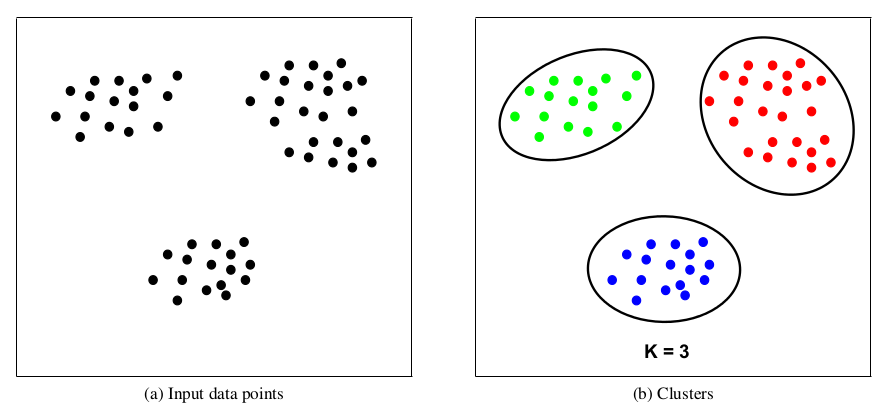
\includegraphics[scale=0.4]{figures/kmeansClust.png}
\caption{\textbf{\textit{k}-Means Clustering}. Example data points, and the clusters computed by \textit{k}-means clustering. Figure courtesy~\cite{junejaThesis}.}
\label{fig:kmeansPic}
\end{figure}

\subsection{Support Vector Machines (\textsc{SVM})}
In machine learning, classification task is a very common task. There are two types of classification tasks in machine learning:
\begin{itemize}
\item \textbf{Supervised Learning.} It is a task of inferring a function from \textit{supervised} training training data. The training data consists of training examples which are pair of an input vector and a desired output label.
\item \textbf{Unsupervised Learning.} This type of learning is used to draw inferences from the datasets consisting of input data without label information. For example, cluster analysis which is used to find the hidden patterns in data.
\end{itemize}

Support Vector Machines is a popular and powerful classification learning tool. It comes under supervised learning tasks. i.e. it learns from a given set of labeled training data and predicts  the label for an unseen test datum. We will explain SVMs for two-class case, which is also called as a ``binary'' classifier. The basic idea behind a linear classifier is to separate the given D-dimensional data points with a $(D − 1)$ dimensional hyperplane. For a given set of points, there may exist multiple hyperplanes which can separate the data (Figure 2.6(a)). The best classifier of all these hyperplanes is the one which provides the maximum separation of the data points (Figure 2.6(b)). It essentially means that the best hyperplane should maximize the distance between the nearest points on both sides of the hyperplane (nearest points to the hyperplane from each class). This distance is defined as the ``margin'', and the SVM selects the hyperplane with the maximum margin. The hyperplane obtained is called maximum-margin hyperplane and the linear classifier is called maximum-margin classifier.

Given a set of n labelled training samples,

\begin{equation}
S =\left\lbrace \left\lbrace x_i ; y_i \right\rbrace | \quad x_i \in D , y_i \in \left\lbrace −1, 1 \right\rbrace \right\rbrace _{i=1}^n
\end{equation}

where, $x_i$ is the $D$-dimensional data point, $y_i$ represents the class to which the $x_i$ belongs.

A separating hyperplane with w as the normal vector, can be written as
\begin{equation}
{w^T}x + b = 0
\end{equation}

Here, $b$ is called the bias term, $\frac{b}{\|w\|}$ gives the perpendicular distance from the origin to the hyperplane. Our goal is to find the $w$ and $b$, such that the ``margin'' is maximized. We can select two parallel hyperplanes which separate the data and are as far as possible (Figure 2.6). These hyperplanes can be written as follows:

\begin{equation}
{w^T}x + b = 1 , \quad
{w^T}x + b = -1
\end{equation}

Now, the distance between the two parallel hyperplanes is $\frac{2}{\|w\|}$. Since the distance needs to be maximised, it translates to minimizing $\|w\|$ . Since we do not want any data points falling in between the two parallel hyperplanes, the following constraints are added:

\begin{equation}
{w^T}x_i + b \geq 1 \qquad \forall x_i \quad s.t \quad y_i = 1
\end{equation}
\begin{equation}
{w^T}x_i + b \leq 1 \qquad \forall x_i \quad s.t \quad y_i = -1
\end{equation}

The two constraints can be combined and rewritten as:

\begin{equation}
y_i(w^{T}x_i + b) \geq 1 \qquad \forall x_i
\end{equation}

We can substitute $\|w\|$ with $\frac{1}{2}\|w\|^2$, without changing the solution, this makes the optimization problem easier to solve. The optimization problem can now be written in primal form as:

\begin{equation}
\begin{split}
\operatornamewithlimits{argmin}_{w, b}\frac{1}{2} \|w\|^2
\qquad subject\quad to \qquad y_i(w^{T}x_i + b) \geq 1 \forall x_i
\end{split}
\end{equation}

\subsection{Bag of Words Method}
The bag of words model in computer vision is inspired from the bag of words model in Natural Language Processing where documents are represented as an unordered collection of words. But in Bag-of-Visual-Words downplays the role of order of words and classifies based on a histogram of the frequency of visual words. The typical bag-of-visual words features consist following steps:
\begin{itemize}
\item Extracting local image features (\textit{e.g.} \textsc{SIFT}, \textsc{HOG}).
\item Visual Words Vocabulary generation. (\textit{e.g.} by \textit{k}-means clustering)
\item Encoding and Spatial Histogram Generation
\item Off-the-self classifier learning on the image descriptors (\textit{e.g.} \textsc{SVM})
\end{itemize}

\subsubsection{Extracting Local Image Descriptors}
The first step is to compute the local features, which captures the local characteristics of an image. In our work, we use \textsc{SIFT} descriptors. These descriptors are extracted at a dense  grid of points. At each point on the dense grid, the \textsc{SIFT} descriptors are computed over multiple circular support patches. The multiple descriptors  are computed at each point to allow for scale variation between images.

\subsubsection{Generating a Codebook}
Once the local image descriptors are computed, the next step is to cluster the local descriptors into a visual words' codebook. A codebook is also known as ``vocabulary" of visual words, which analogous to the dictionary in text domain. The idea behind a codebook is that an image can be represented in terms of these visual words. \textit{k}-means clustering  is a popular method to construct a vocabulary of visual words. A set of random descriptors from a subset of the Training set images is used to construct the visual vocabulary. The number of visual words is a parameter that depends on the dataset, and is generally determined experimentally.

\subsubsection{Histograms Creation}
After learning the vocabulary above, each image is then represented as a bag-of-visual words. Each local descriptor $x_i$ is encoded by the nearest visual word in the Euclidean space. An Euclidean space can be denoted by:

\begin{equation}
c_i = \operatornamewithlimits{argmin}_k \|x_i - \mu_k\|^2
\end{equation}

After getting the encodings for all the local descriptors in an image, it is described by a vector (or histogram) that stores the distribution of all the visual words. The size of the histogram is equal to the vocabulary size, where each bin corresponds to a visual word. The final descriptor of an image is a concatenation of the encodings of different spatial regions into a single vector. Note that the histograms of each region are individually normalized before concatenation. The distance between the two vectors reflects the extent to which the images contain similar appearance and the extent to which the appearances correspond in their spatial layout.

\subsubsection{Model Learning}
After getting the image descriptors, the aim is to learn models (classifiers) for the different classes. \textsc{SVM} is a commonly used classifier in \textsc{BoW} steps. For each class, a separate SVM is learned which can predict whether an unseen image belongs to that particular class or not. For training an SVM for a particular class, the descriptors of the images belonging to that class act as positive data points for the SVM, and descriptors of rest of the
images act as negative data points. The set of these positive and negative images is also referred to as the Training Set, while the set of unseen images whose classes are to be predicted, is referred to as the Test Set.

\section{Deep Learning and Recurrent Neural Networks}
\label{sec:deep}

\subsection{Recurrent Neural Networks}
Recurrent Neural Networks (\textsc{RNN}s) are inspired from the way a human thinks. Everytime, humans don't start thinking from the scratch. They build upon the knowledge which persists across time. Traditional Neural Networks can't do this, for example a traditional neural network can't predict an event based on its past experiences. \textsc{RNN}s, however address this issue, which have loops in them, which allow the information to persist.

\begin{figure}[h]
\centering
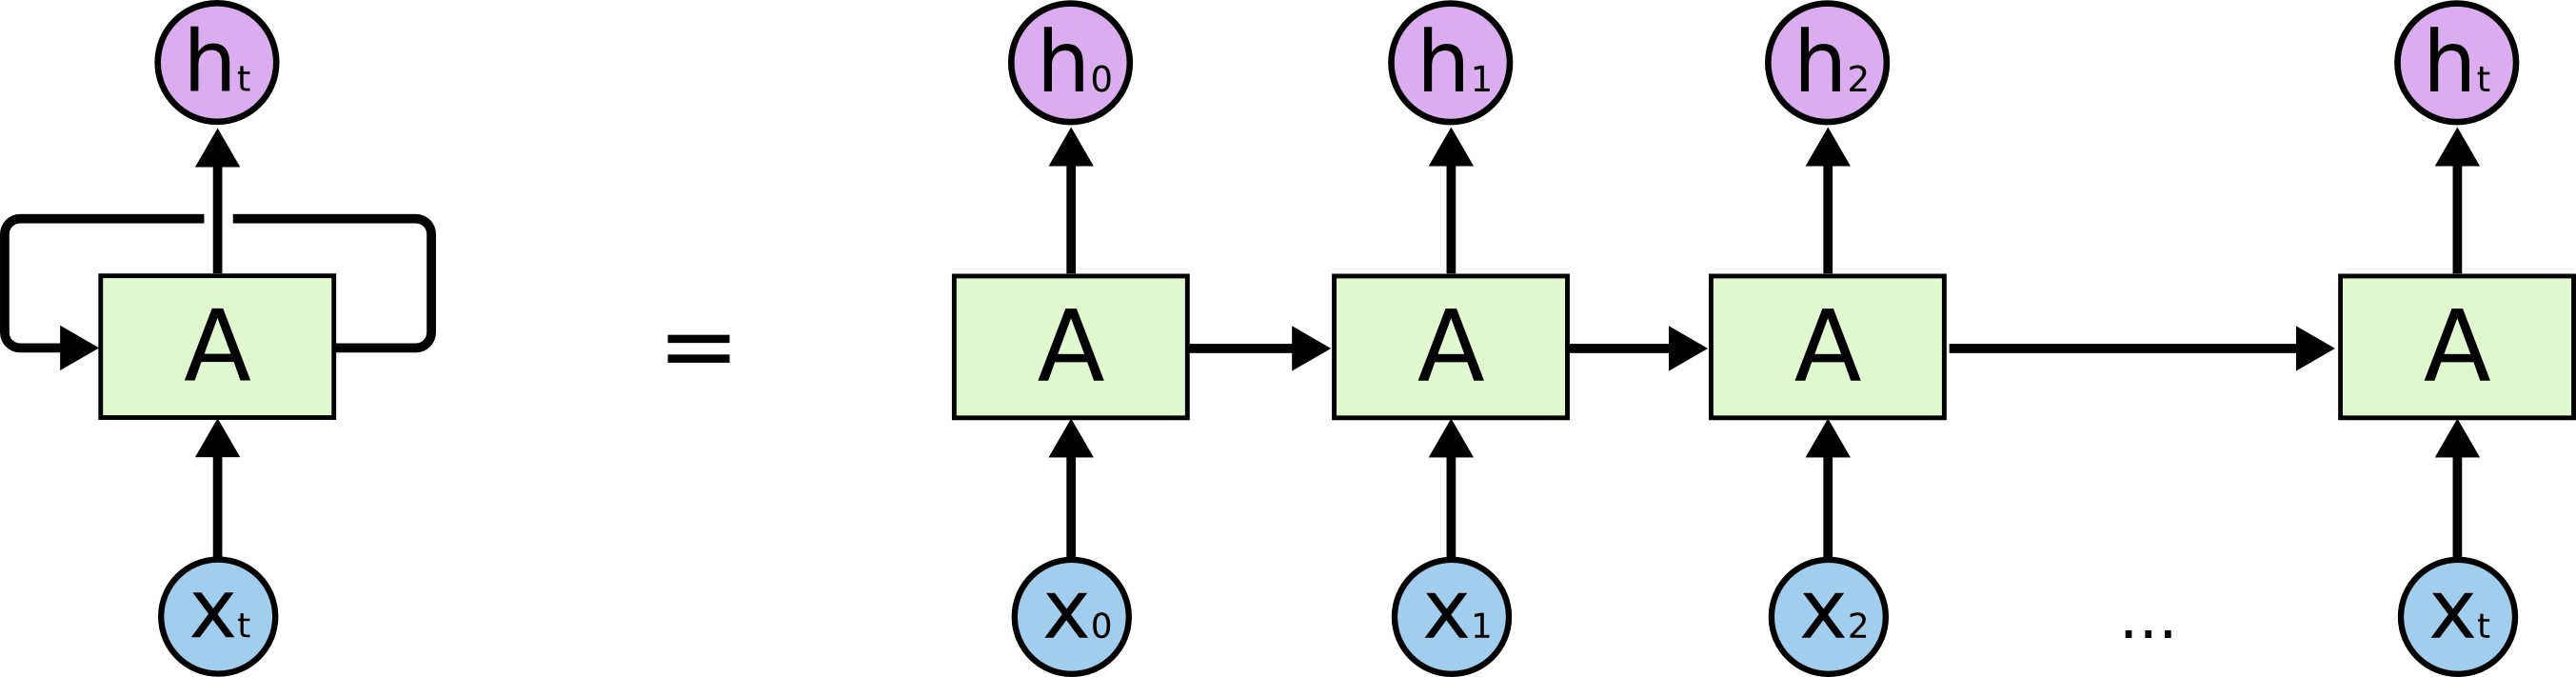
\includegraphics[scale=0.4]{figures/RNN-unrolled.png}
\caption{A recurrent neural network, unrolled.~\cite{colahSite}}
\label{fig:unrollRNN}
\end{figure}


As shown in Figure~\ref{fig:unrollRNN}, \textsc{RNN}s, when unrolled reveal a chain-like nature and are intimately related to sequences and list. One of the appeals of the \textsc{RNN}s is the idea that they might be able to connect previous information to the present task, such as using previous video frames might inform the understanding of the present frame. Sometimes, we only need to look at recent information to perform the present task. For example, consider a language model trying to predict the next word based on the previous ones. If we are trying to predict the last word in ``the clouds are in the sky," we don’t need any further context – it’s pretty obvious the next word is going to be sky. In such cases, where the gap between the relevant information and the place that it’s needed is small, RNNs can learn to use the past information. But there are also cases where we need more context. Consider trying to predict the last word in the text ``I grew up in France… I speak fluent French." Recent information suggests that the next word is probably the name of a language, but if we want to narrow down which language, we need the context of France, from further back. It’s entirely possible for the gap between the relevant information and the point where it is needed to become very large.

\noindent\textbf{Long Short Term Memory Networks.} As we have seen above, \textsc{RNN} are capable of persisting an information over a small timesteps or gap but it can't do that over a longer timesteps. Hence, Hochreiter and Schmidhuber introduced Long Short Term Memory (\textsc{lstm}) networks. These are special kind of \textsc{RNN}s which are capable of learning the long-term dependencies.

All recurrent neural networks have the form of a chain of repeating modules of neural network. In standard RNNs, this repeating module will have a very simple structure, such as a single \textit{tanh} layer.

\begin{figure}[h]
\centering
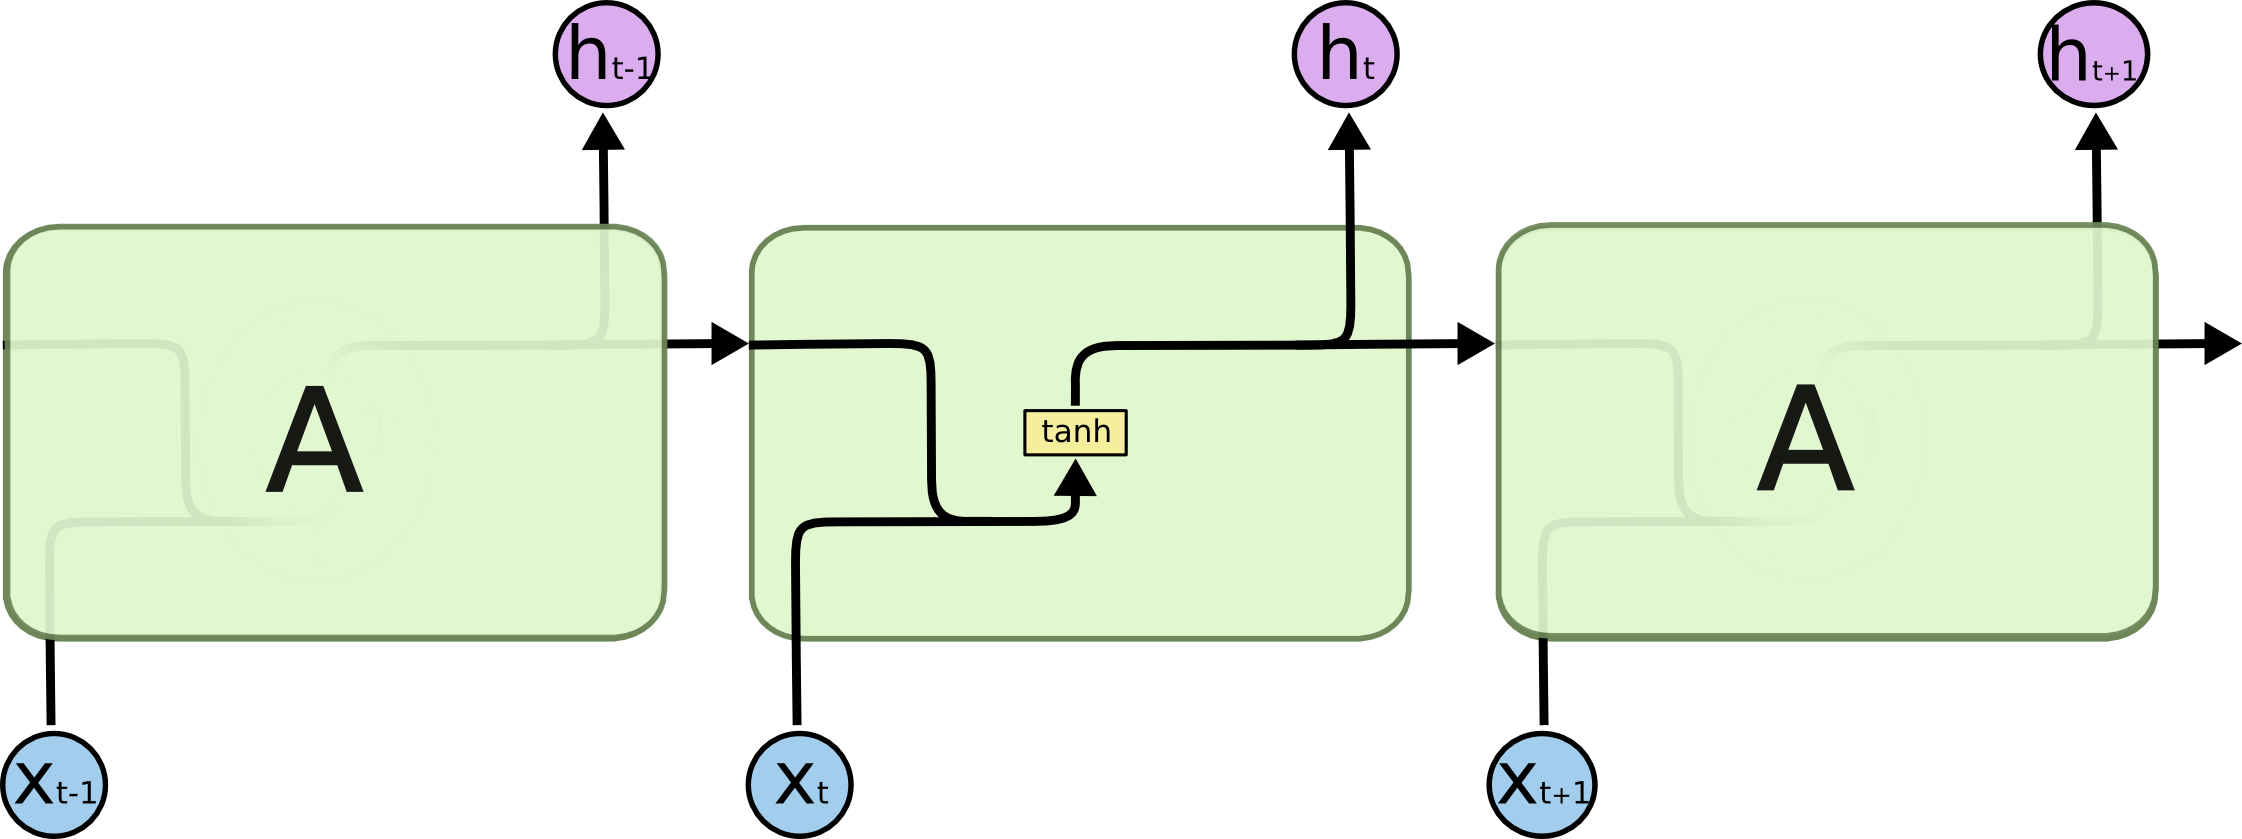
\includegraphics[scale=0.4]{figures/LSTM3-SimpleRNN.png}
\caption{The repeating module in a standard \textsc{RNN} contains a single layer~\cite{colahSite}}
\label{fig:simpleRNN}
\end{figure}

\textsc{LSTM}s also have this chain like structure, but the repeating module has a different structure. Instead of having a single neural network layer, there are four, interacting in a very special way. Key to the \textsc{LSTM} is the cell state, the horizontal line running through  the top of the diagram. The cell state is like a conveyor belt. It runs straight down the entire chain, with minor linear interactions, which helps the information to flow along it unchanged. The \textsc{LSTM} cell have the ability to remove or add information to the cell state, carefully regulated by structures called gates. Gates are a way to optionally let information through. They are composed out of sigmoid neutral net layer and a pointwise multiplication operation. These gates allows \textsc{LSTM} memory cells to store and access information over long period of time, thereby avoiding the vanishing gradient problem. 

For example, as long as the input gate remains closed (i.e. has an activation close to 0), the activation of the cell will not be overwritten by the new inputs arriving in the network, and can therefore be made available to the net much later in the sequence, by opening the output gate.
The preservation over time of gradient information by LSTM is illustrated in Figure~\ref{fig:memGates}.

\begin{figure}[h]
\centering
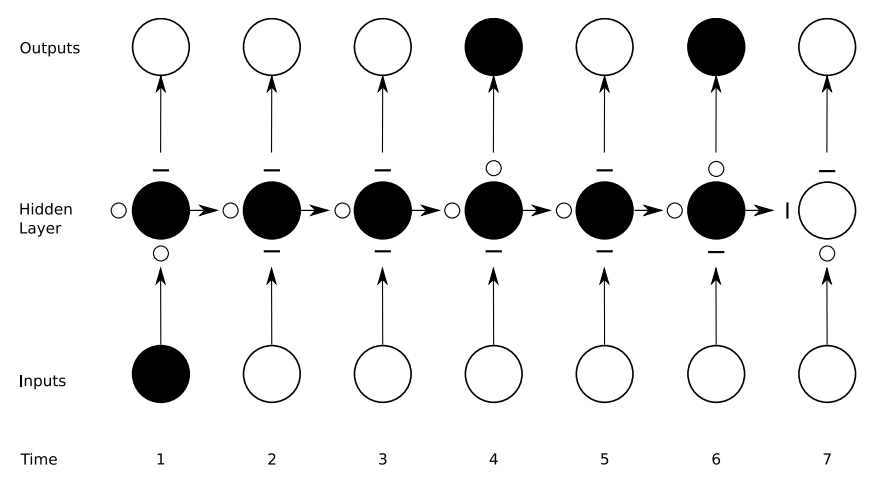
\includegraphics[scale=0.4]{figures/memoryGates.png}
\caption{\textbf{Preservation of gradient information by \textsc{LSTM}.} The state of the input, forget, and output gate states are displayed below, to the left and above the hidden layer node, which corresponds to a single memory cell. For simplicity, the gates are either entirely open (`$O$') or closed (`-'). The memory cell `remembers' the first input as long as the forget gate is open and the input gate is closed, and the sensitivity of the output layer can be switched on and off by the output gate without affecting the cell.~\cite{gravesThesis}}
\label{fig:memGates}
\end{figure}


\noindent\textbf{\textsc{LSTM} in Action} As it can be seen in the Figure~\ref{fig:lstmRNN}, there are four interacting layers in a cell. We will go through each layer one by one. In Figure~\ref{fig:lstmRNN}, (i) step, \textsc{LSTM} has to decide upon the information which needs to be thrown out from the cell state. This decision is made by a sigmoid layer called the ``forget gate layer''. A $1$ represents ``completely keep this'' while $0$ represents ``completely get rid of this''. The (ii) step decides what new information we're going to store in the cell states. This has two parts, a) a sigmoid layer called the ``input gate layer'' decides which values we'll update and b) a \textit{tanh} layer creates  a vector of new candidate values that could be added to the state. In (iii) step, we will combine these two to create an update to the state. In the (iv) and final step we decide what we're going to output. Then, we run a sigmoid layer which decides what parts of the cell state we’re going to output. Then, we put the cell state through \textit{tanh} (to push the values to be between ${-1}$ and $1$) and multiply it by the output of the sigmoid gate, so that we only output the parts we decided to.    

\begin{figure}[h]
\centering
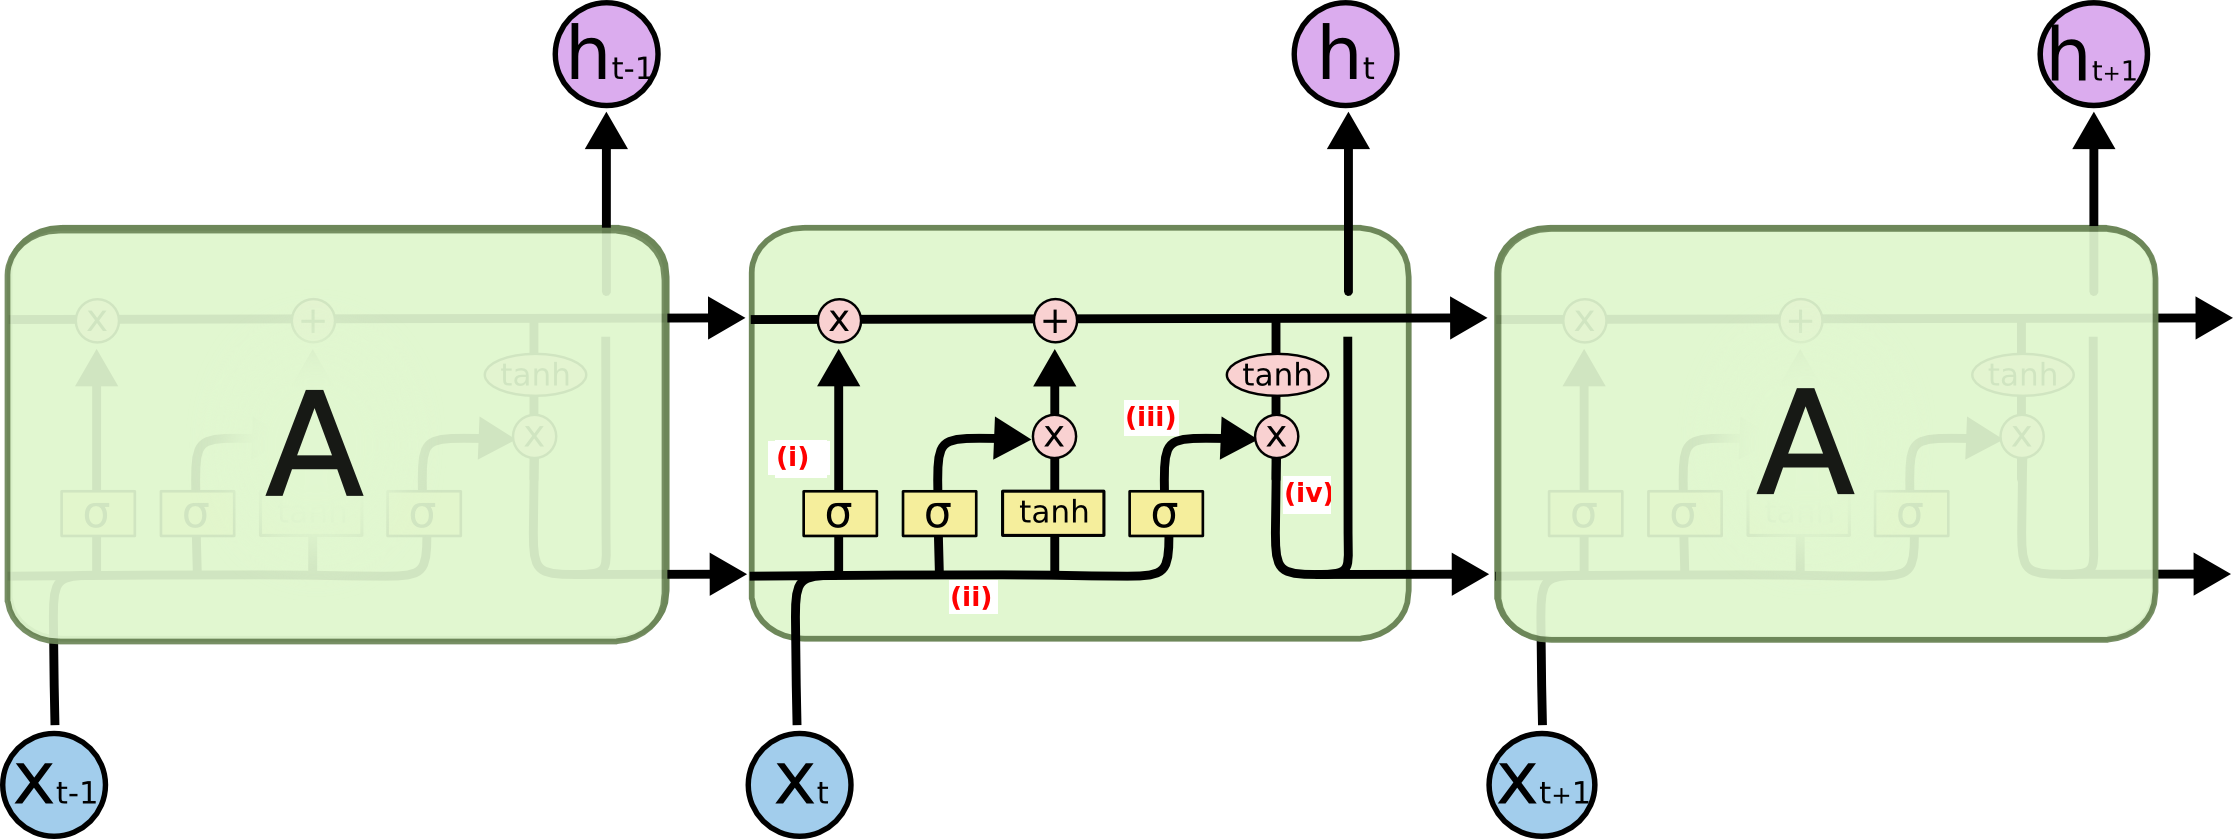
\includegraphics[scale=0.4]{figures/LSTM3-chain_1.png}
\caption{The repeating module in a standard \textsc{RNN} contains four interacting layers.~\cite{colahSite}}
\label{fig:lstmRNN}
\end{figure}

\textsc{LSTM} has been applied to various real-world problems, such as protein secondary structure prediction~\cite{Hochreiter07}, music generation~\cite{Music02}, reinforcement learning ~\cite{Bakker02} and speech recognition and handwriting recognition~\cite{GravesLFBBS09}. As would be expected, its advantages are most pronounced for problems requiring the use of long range contextual information.